\documentclass[12pt, a4paper]{article}
\usepackage[spanish]{babel}
\usepackage[utf8]{inputenc}
\usepackage{graphicx}
\usepackage{geometry}
\usepackage{fancyhdr}
\usepackage{float}
\usepackage{titling}
\usepackage{hyperref}
\usepackage{url}




% Márgenes
\geometry{a4paper, margin=2.5cm}

% Encabezado y pie de página
\pagestyle{fancy}
\fancyhf{}
\rhead{
\includegraphics[height=1.2cm]{images/logo-usm.png}}
\lhead{Grupo 19\\Visualización de Datos}
\rfoot{Página \thepage}

% Configuración del logo en portada
\pretitle{
  \begin{center}
  \vspace{1cm}
  
\includegraphics[width=0.5\textwidth]{images/logo-usm.png}\\
  \vspace{1.5cm}
  \LARGE
}
\posttitle{\end{center}}

% Título del informe
\title{Informe: Tecnología en la Vida Cotidiana}
\author{Felipe Campaña, Javier Gómez, Matias Elgueta}
\date{\today\\[2cm]}

\begin{document}
\maketitle

% ---------------------------------------------------------------------------------
\section*{Criterios de Selección}
\begin{itemize}
    \item Criterio 1: Porcentaje de uso de internet en el mundo
    \item Criterio 2: Porcentajes de contratación de fibra en el mundo (Top 10)
    \item Criterio 3: Horas en redes sociales por país
    \item Criterio 4: Evolución de clientes de Telecomunicación
    \item Criterio 5: **
    \item Criterio 6: **
\end{itemize}

% ---------------------------------------------------------------------------------
\section*{Análisis por Integrante}

% ===================== FELIPE CAMPAÑA =====================
\subsection*{Integrante 1: Felipe Campaña}

\subsubsection*{Criterios Seleccionados}
\begin{itemize}
    \item Porcentaje de uso de internet en el mundo.
    \item Porcentajes de contratación de fibra en el mundo (Top 10).
\end{itemize}

\subsubsection*{Justificación: Contratación de Fibra Óptica Fija}
Este indicador representa cuántas personas por cada 100 habitantes tienen acceso a Internet mediante conexiones de alta velocidad y calidad. 

\begin{itemize}
    \item Evalúa el nivel de infraestructura tecnológica en cada país.
    \item Refleja el grado de modernización digital más allá de la simple conectividad.
    \item Relacionado con la capacidad de ofrecer servicios como streaming, teletrabajo, etc.
\end{itemize}

\subsubsection*{Justificación: Acceso a Internet en la Población}
Este indicador señala el porcentaje de personas que utilizan Internet, sin importar el tipo de conexión.

\begin{itemize}
    \item Entrega una visión inclusiva del uso digital básico en cada país.
    \item Identifica regiones con barreras fundamentales de conectividad.
    \item Refleja impacto de políticas públicas y accesibilidad económica.
\end{itemize}

\subsubsection*{Gráfico 1: Uso de internet de las personas en el mundo}
\begin{figure}[H]
    \centering
    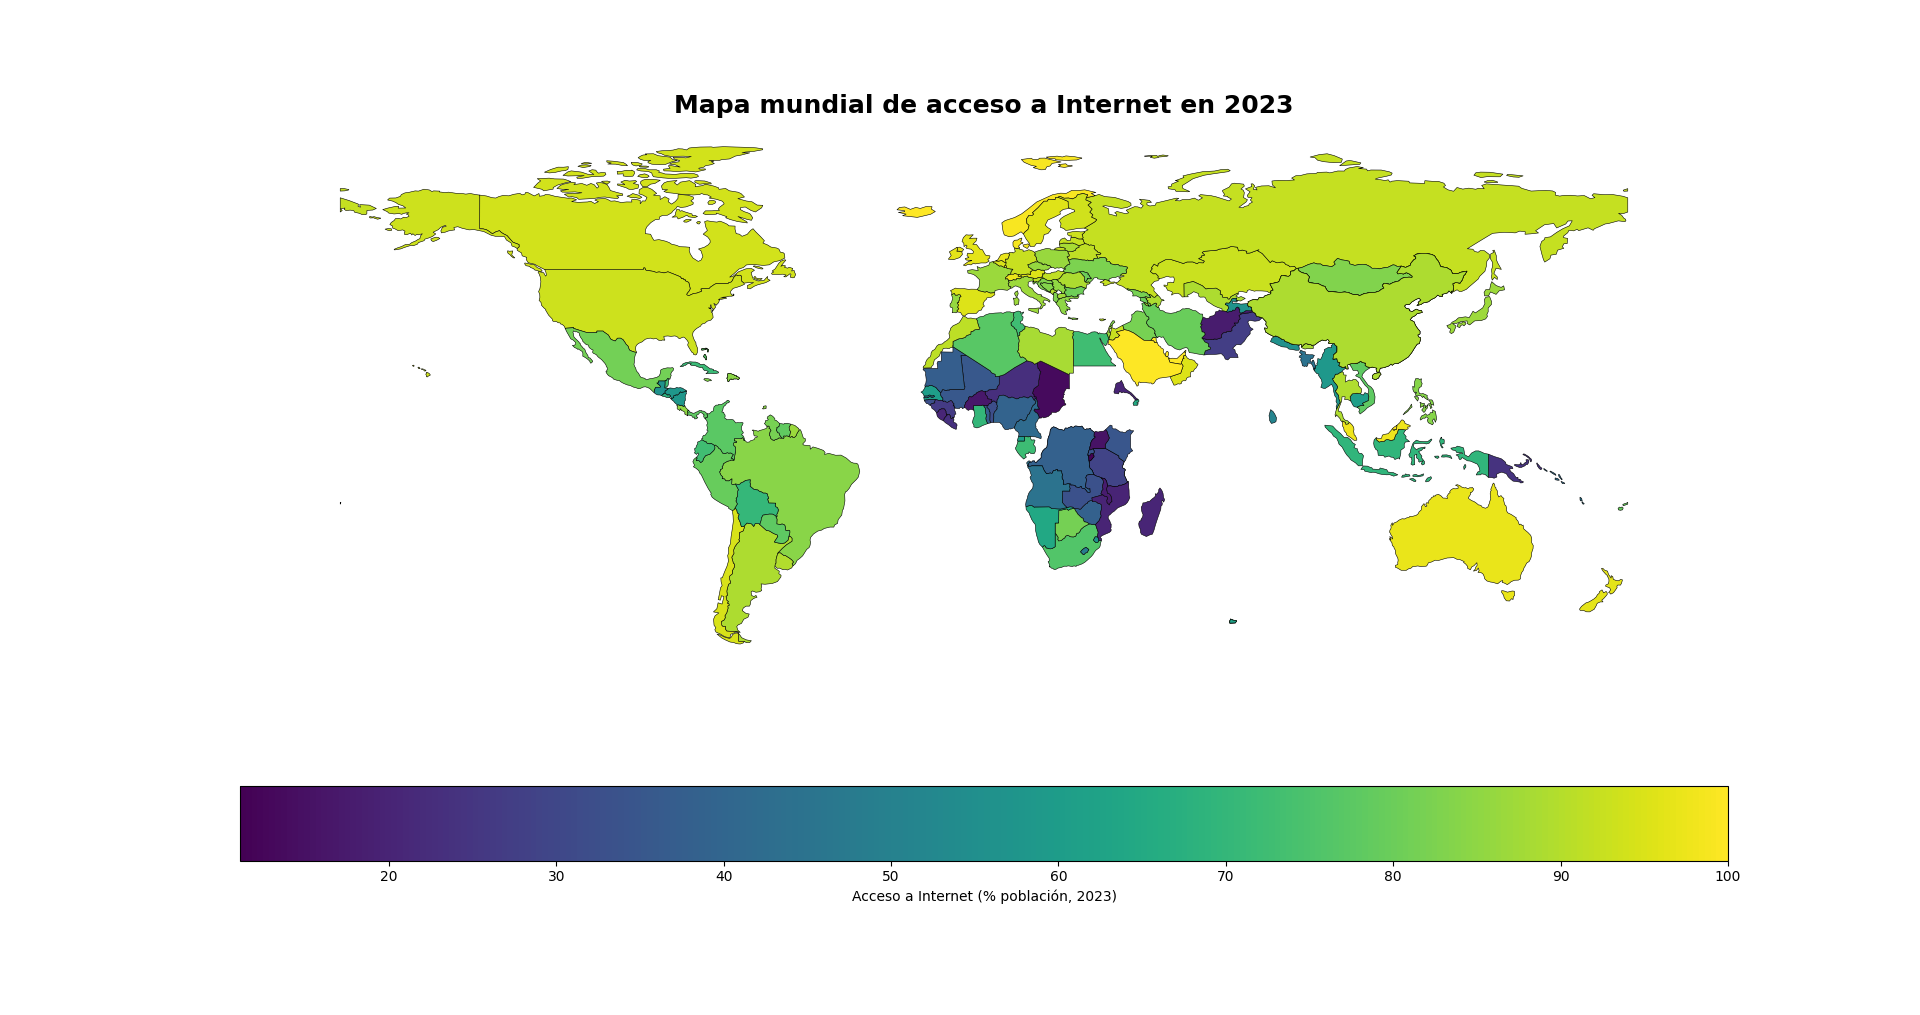
\includegraphics[width=0.85\textwidth]{images/Grafico_uso_de_internet_FC.png}
    \caption[1]{Fuente: Elaboración propia con datos de \href{https://data.worldbank.org}{World Bank} 
    (\url{https://data.worldbank.org/indicator/IT.NET.USER.ZS}).}
\end{figure}

\textbf{Conclusión:}
\begin{itemize}
    \item Muestra un panorama global del acceso digital: Europa, Oceanía y partes de Asia y América alcanzan más del 80\% de cobertura poblacional.
    \item África central y algunos países del sudeste asiático presentan niveles muy bajos (<40\%), lo que evidencia una brecha digital persistente.
    \item Países como Sudán, Congo o Yemen están en las zonas más oscuras del mapa, reflejando problemas estructurales en conectividad.
    \item Este mapa destaca diferencias regionales importantes que no necesariamente se reflejan en el gráfico de fibra óptica.
    \item Es una excelente forma de visualizar desigualdades sociales y tecnológicas a escala global.
\end{itemize}

\subsubsection*{Gráfico 2: Top 10 países con mayor porcentaje de fibra contratada}
\begin{figure}[H]
    \centering
    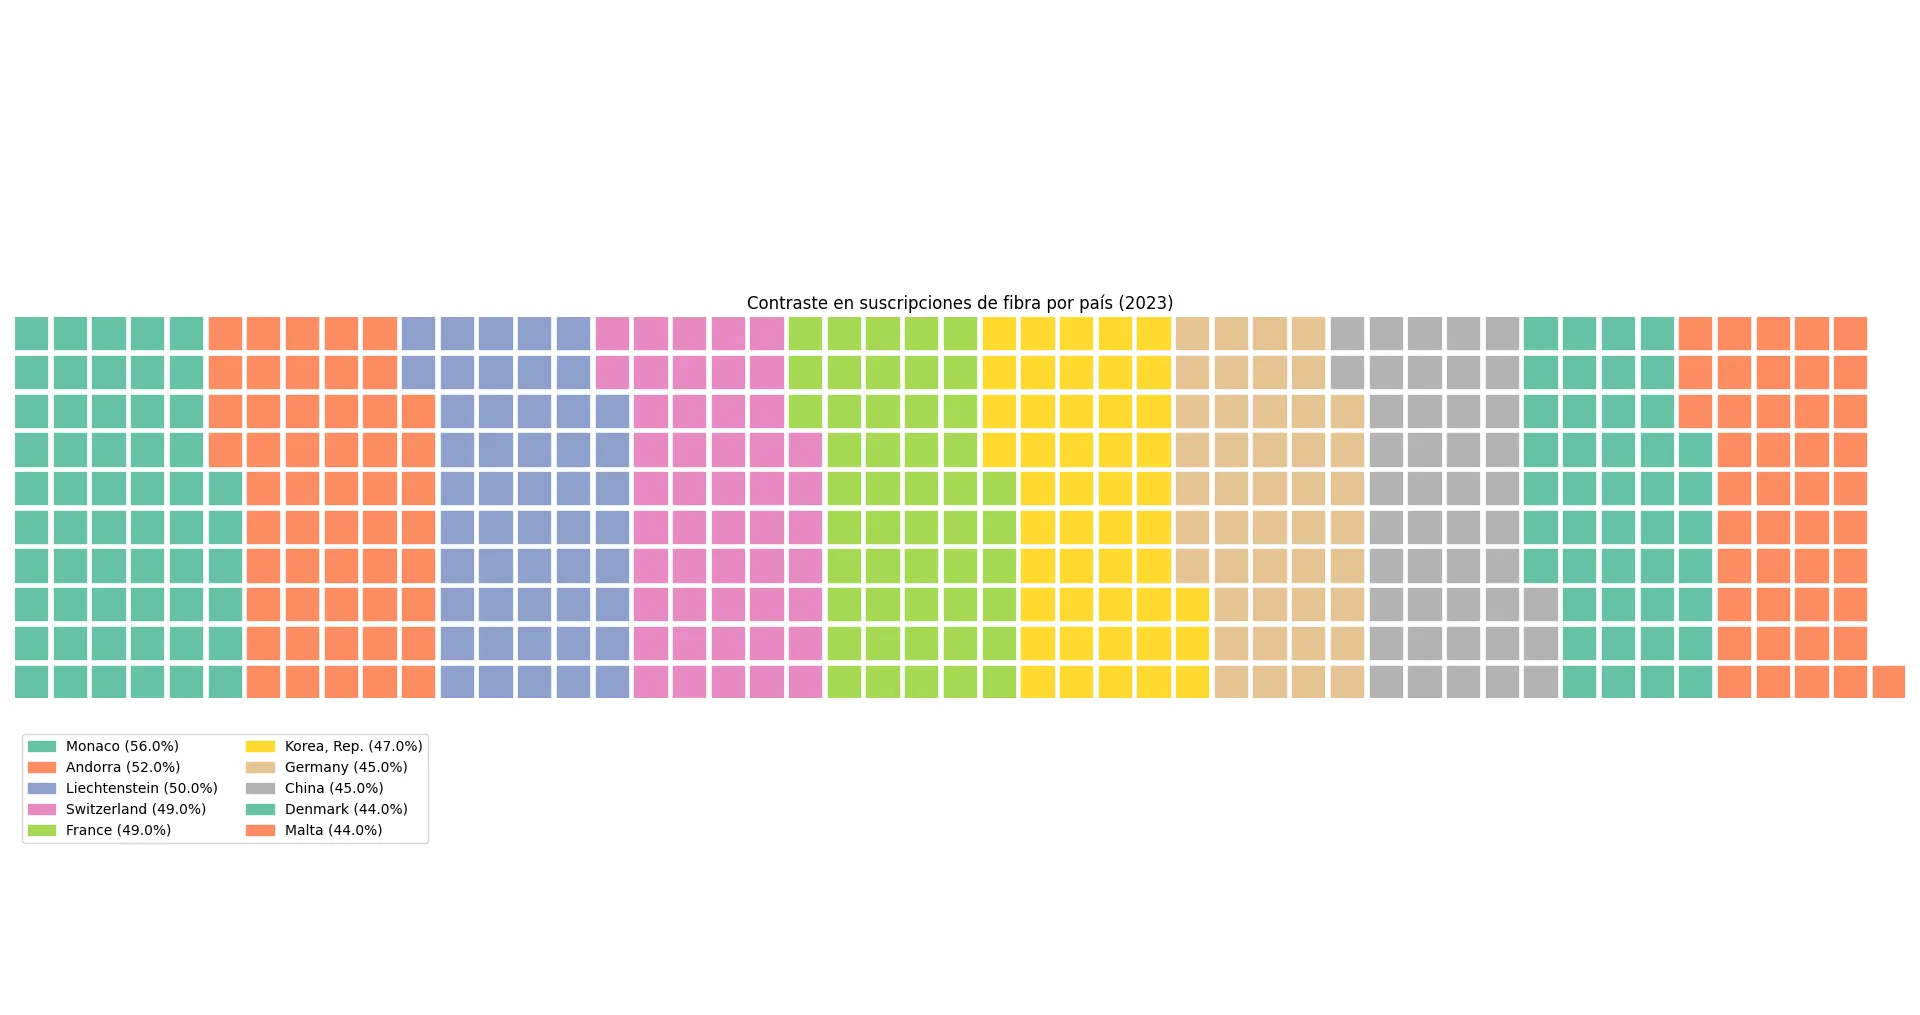
\includegraphics[width=1\textwidth]{images/Grafico_fibra_contratada_FC2.png}
    \caption[2]{Fuente: Elaboración propia con datos de \href{https://data.worldbank.org}{World Bank} 
    (\url{https://data.worldbank.org/indicator/IT.NET.BBND.P2}).}
\end{figure}

\textbf{Conclusión:}
\begin{itemize}
    \item Se observa que países como Mónaco (56\%), Andorra (52\%) y Liechtenstein (50\%) lideran la contratación de fibra en 2023.
    \item Son en general países pequeños, con economías desarrolladas y buena planificación urbana, lo que facilita la instalación de redes avanzadas.
    \item Países como China, Corea del Sur o Alemania también presentan cifras altas, pero no alcanzan el nivel de penetración de los primeros.
    \item El gráfico también muestra países con niveles más bajos, como Malta y Dinamarca (44\%), lo que sugiere diferencias internas incluso en regiones desarrolladas.
    \item Este tipo de visualización permite un contraste claro de adopción tecnológica y pone en evidencia el avance en infraestructura.
\end{itemize}


% ===================== JAVIER GÓMEZ =====================
\newpage
\subsection*{Integrante 2: Javier Gómez}

\subsubsection*{Criterios Seleccionados}
\begin{itemize}
    \item Horas diarias en redes sociales por país.
    \item Contratación de telecomunicaciones en Chile.
\end{itemize}

\subsubsection*{Justificación: Horas diarias en Redes Sociales}
Permite segmentar audiencias e identificar poblaciones con alto uso digital, útil para campañas publicitarias o estudios sociales.

\begin{itemize}
    \item Instituciones educativas pueden actuar frente a exceso de uso en estudiantes.
    \item Posible vínculo con salud mental o rendimiento académico.
\end{itemize}

\subsubsection*{Justificación: Contratación de Telecomunicaciones}
Revela qué compañías dominan la provisión de internet, destacando posibles monopolios u oligopolios.
\begin{itemize}
    \item Revela si los consumidores valoran precio, velocidad o cobertura.
\end{itemize}

\subsubsection*{Gráfico 3: Horas diarias en redes sociales por país}
\begin{figure}[H]
    \centering
    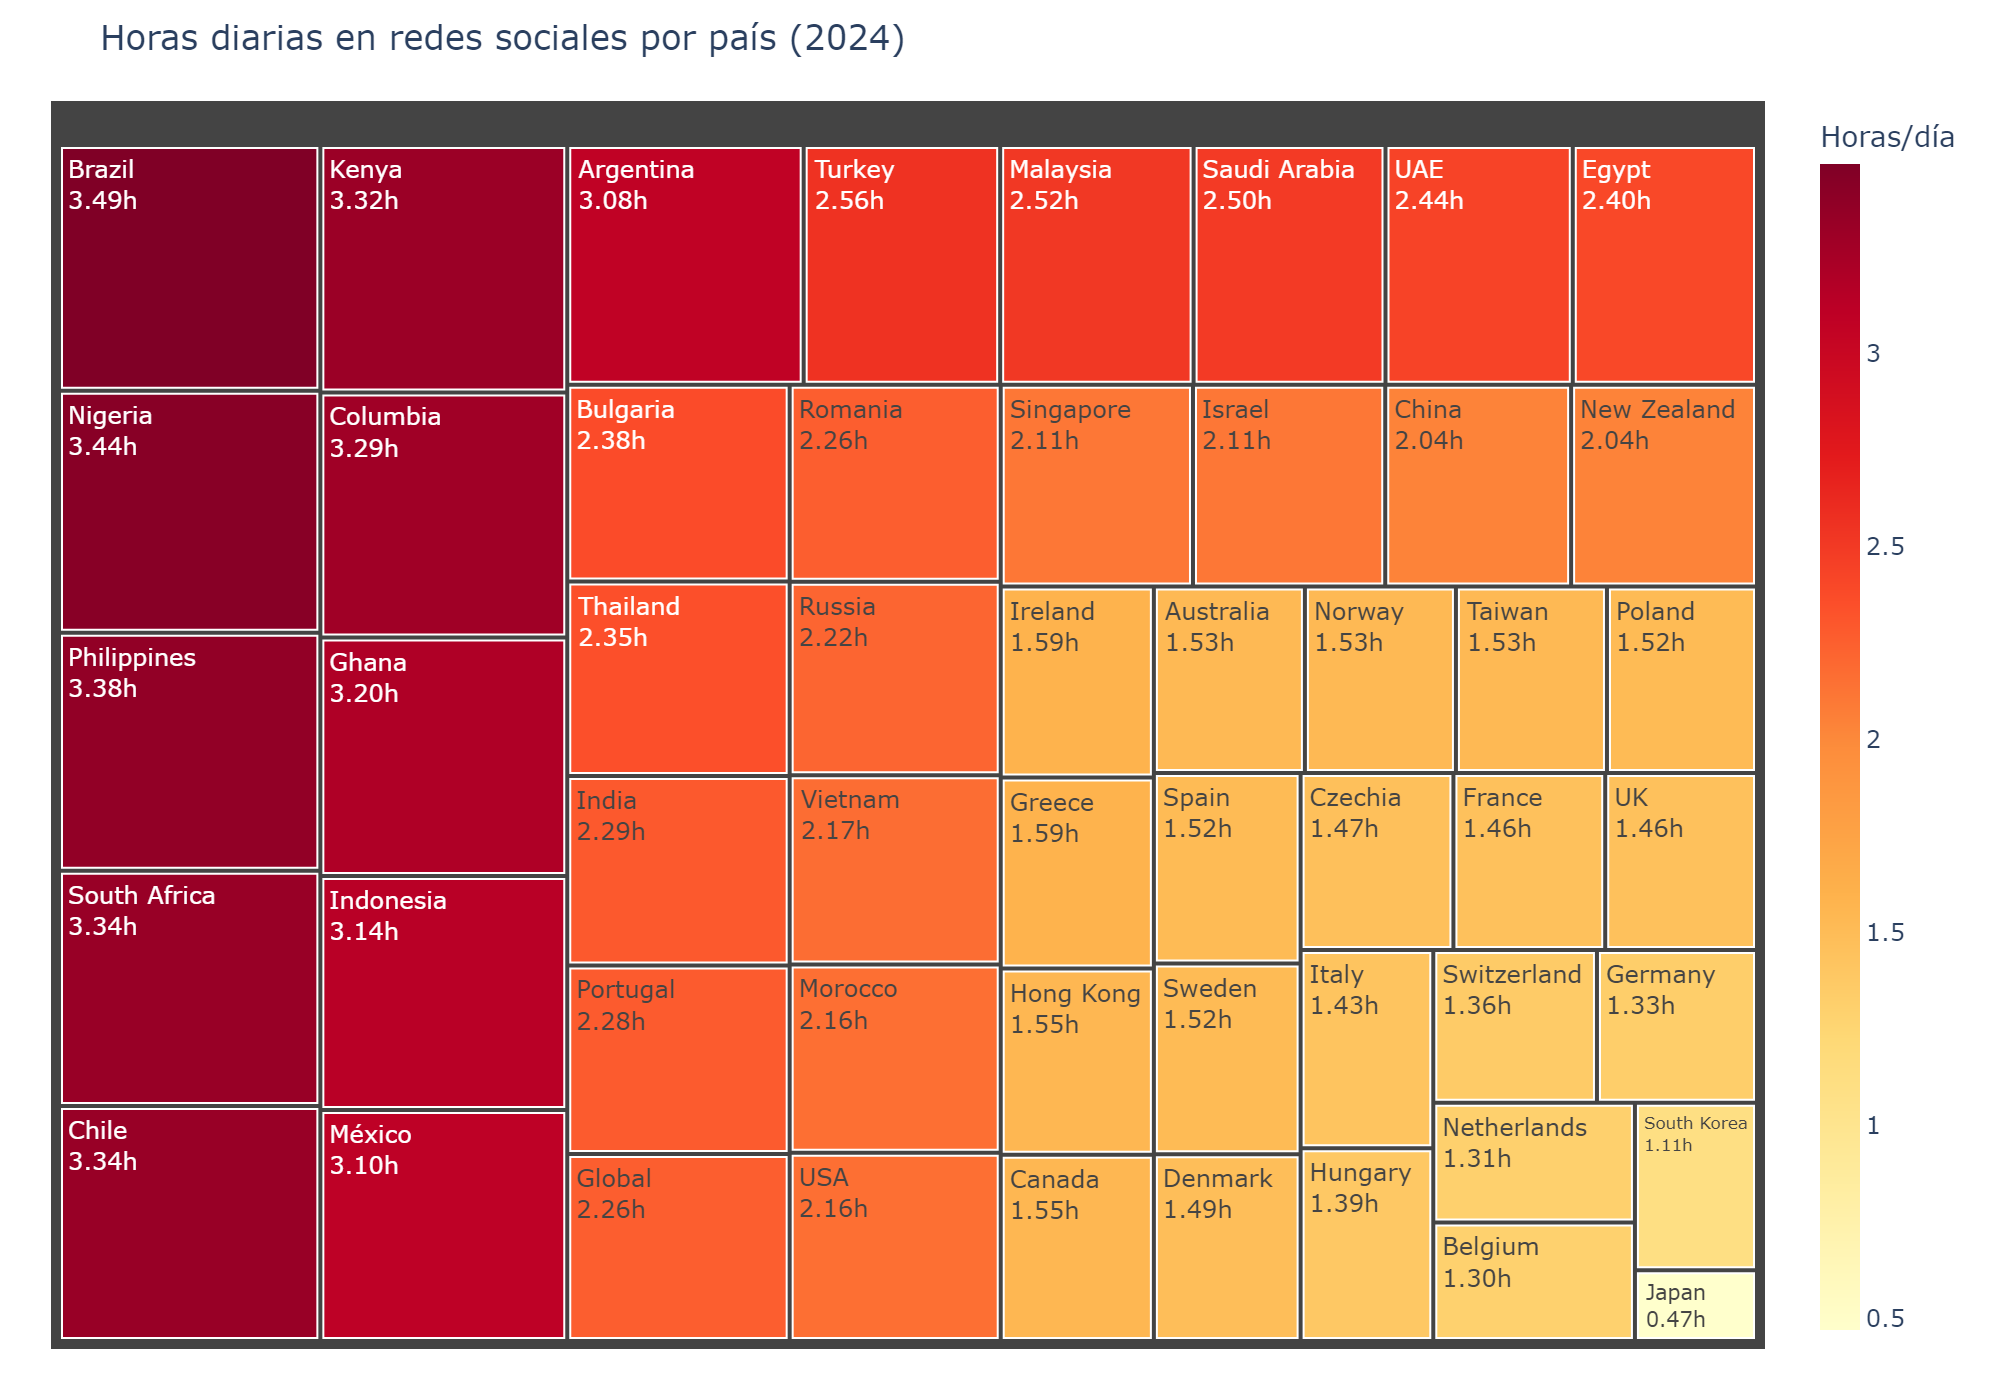
\includegraphics[width=0.85\textwidth]{images/graph1_JG.png}
    \caption{
        Fuente: Elaboración propia con datos de Statista (2024). 
        \textit{Promedio de minutos diarios de uso de redes sociales por los internautas en países seleccionados en el tercer trimestre de 2023}. 
        Recuperado de \url{https://www.statista.com/statistics/270229/usage-duration-of-social-networks-by-country/}
    }
\end{figure}

\newpage
\textbf{Conclusión:}  
\begin{itemize}
    \item Como se puede ver en el gráfico, países como Brasil, Nigeria, Filipinas y Chile lideran el ranking en cuanto a uso diario de redes sociales, con promedios superiores a las 3 horas diarias. En general, los países de América Latina y África muestran un uso bastante elevado, lo que refleja lo presentes que están estas plataformas en la vida cotidiana de sus habitantes.
    \item Por otro lado, en países como Japón, Alemania o Bélgica, el tiempo promedio dedicado a redes sociales es mucho menor. Esto puede estar relacionado con diferencias culturales o incluso con estilos de vida donde quizás se priorizan otras formas de comunicación.
    \item El lector podría encontrar interesante realizar un estudio frente a la relación entre cantidad de horas frente a, por ejemplo, rendimiento académico $\bullet{}\bigcirc{}\bullet{}$
\end{itemize}

\subsubsection*{Gráfico 4: Contratación de telecomunicaciones}
\begin{figure}[H]
    \centering
    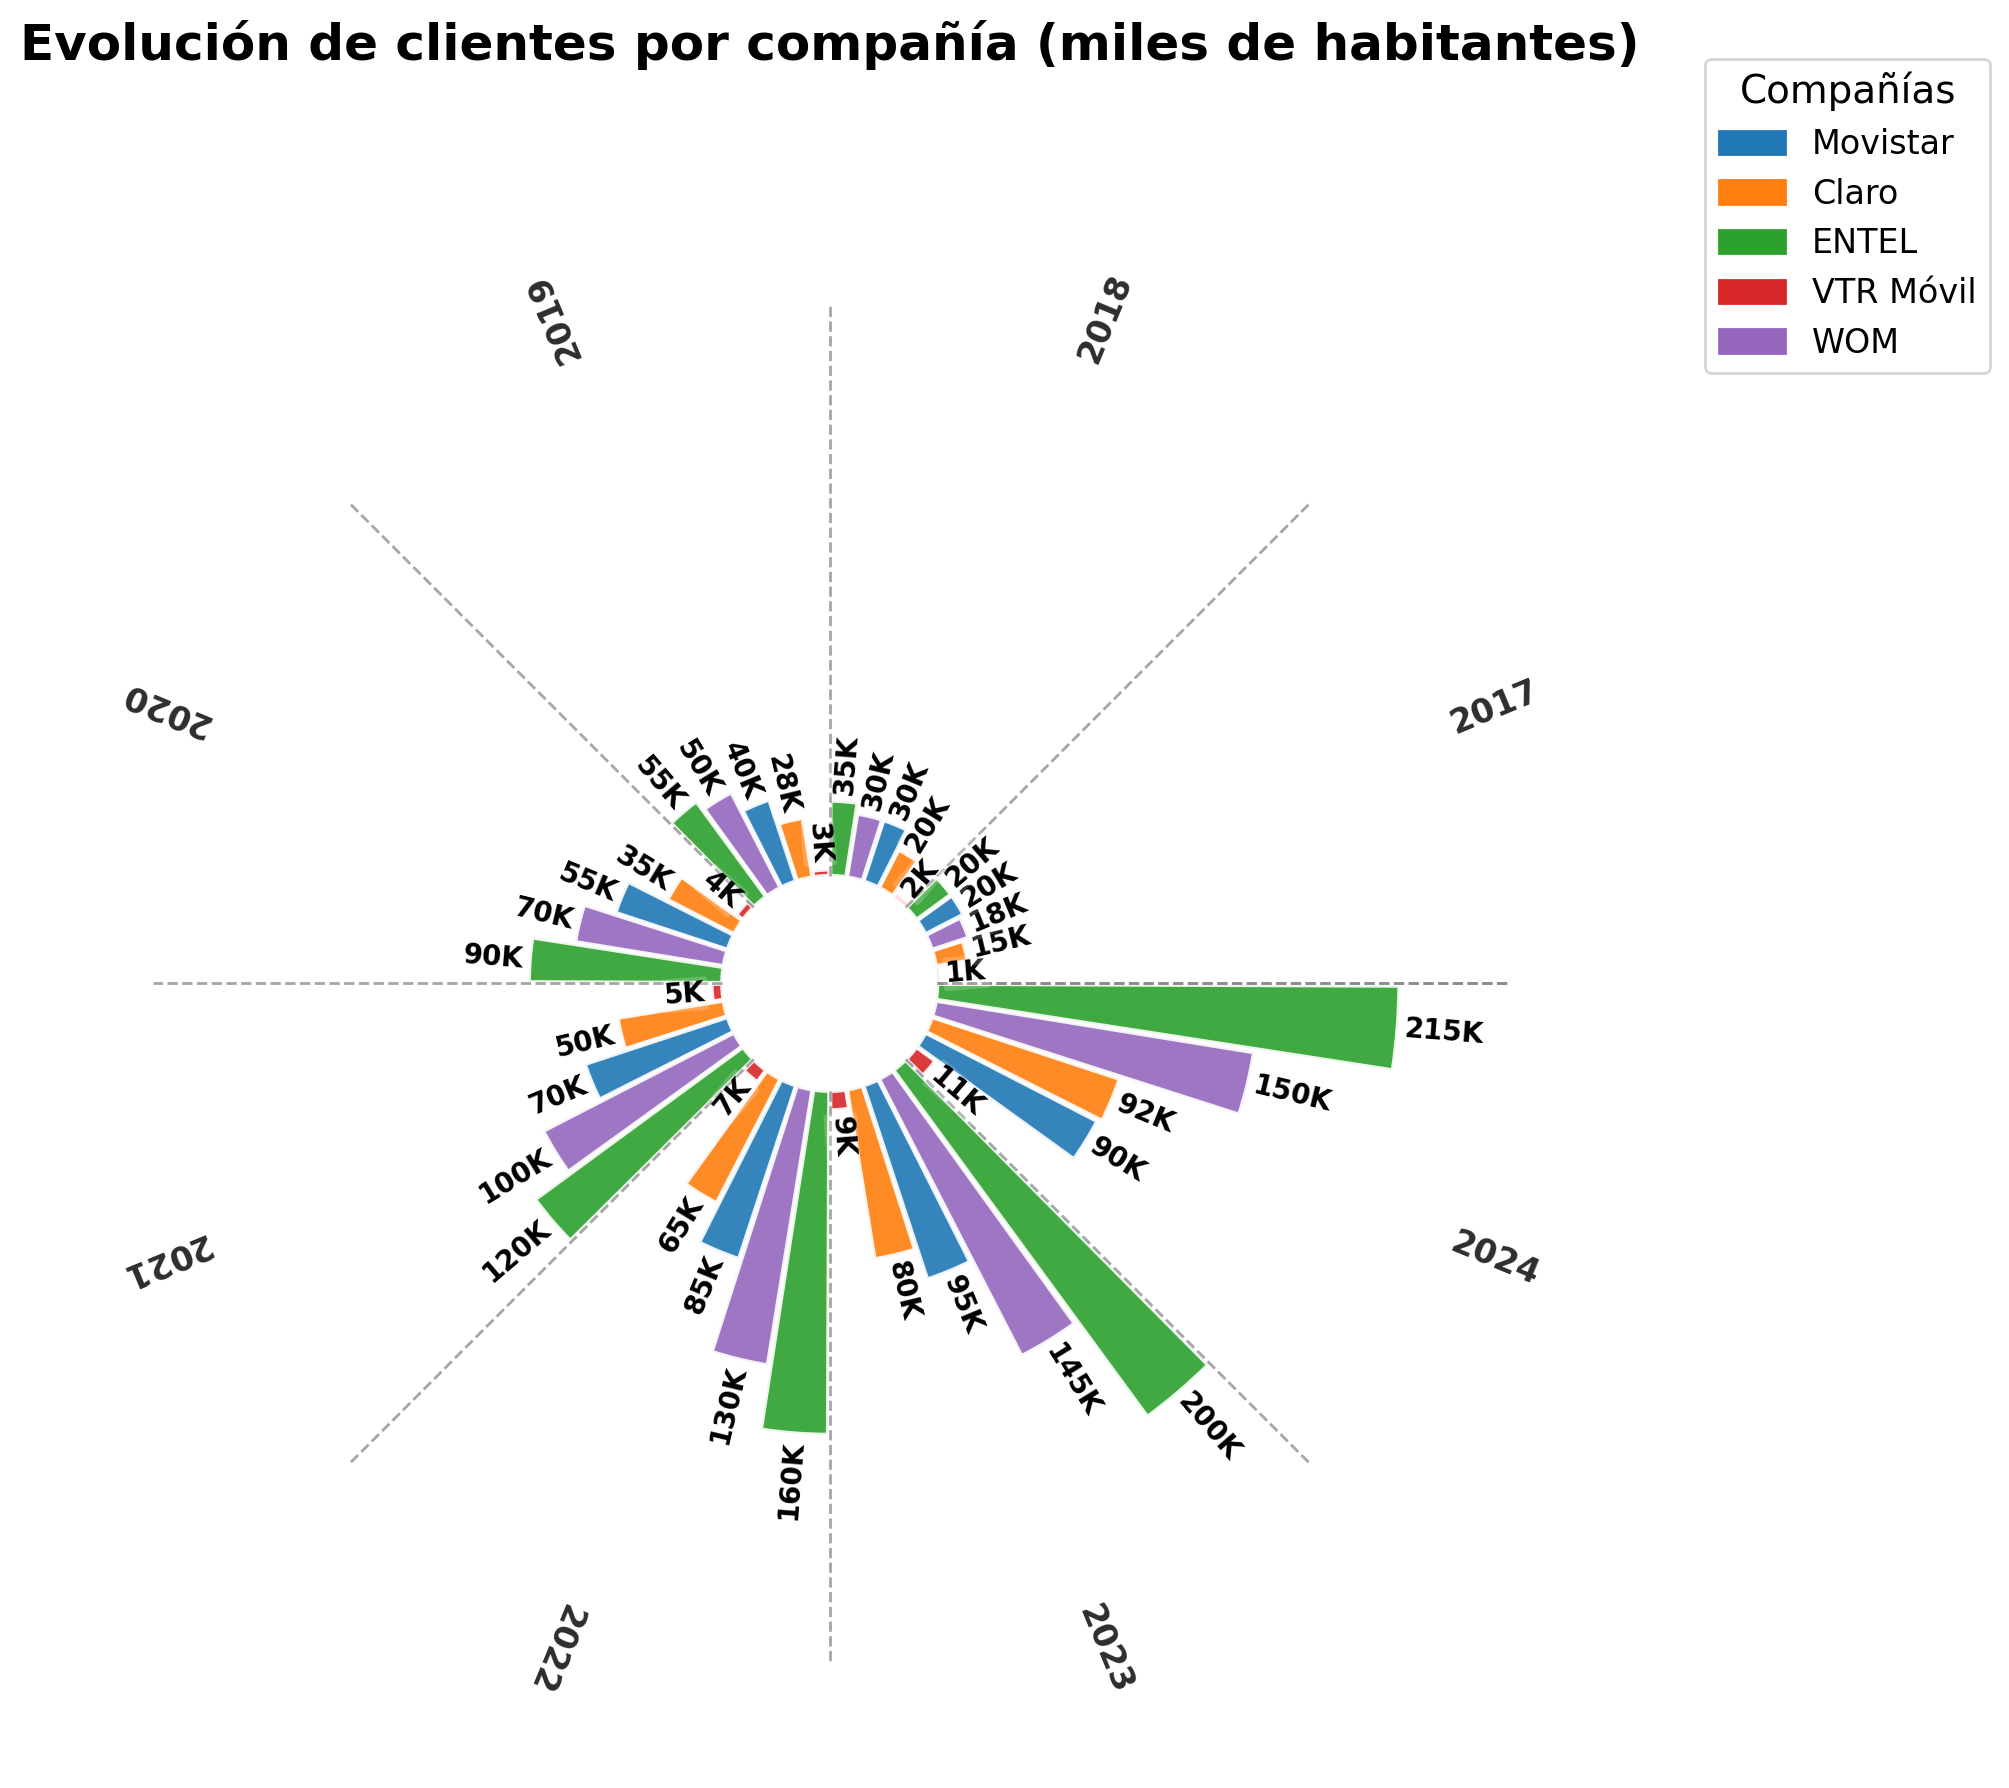
\includegraphics[width=0.85\textwidth]{images/graph2_JG.png}
    \caption{
        Fuente: Elaboración propia con datos de Subsecretaría de Telecomunicaciones (2025), 
        \textit{Informe del Sector Telecomunicaciones: Cierre 2024}, p. 13. 
        Disponible en \url{https://www.subtel.gob.cl/wp-content/uploads/2025/02/Informe_del_Sector_Telecomunicaciones_Dic24.pdf}
    }

\end{figure}


\textbf{Conclusión:}  
\begin{itemize}
    \item Este gráfico muestra la evolución del número de clientes por empresa en los últimos años. Lo más destacable es el aumento significativo de las suscripciones a servicios móviles durante la pandemia \(2020-2021\).
    Durante esos años, varias empresas, como WOM y ENTEL, experimentaron un fuerte crecimiento, probablemente impulsado por la necesidad de mantenerse conectados desde casa, ya sea por trabajo, estudios o simplemente para mantenerse en contacto con los demás.
    \item También es notable cómo algunas empresas han mantenido una base de clientes más estable a lo largo del tiempo, mientras que otras, como VTR Móvil, tienen una participación mucho menor. En 2024, ENTEL se destacó como la empresa con más clientes, superando los 215.000, lo que podría indicar una estrategia comercial sólida o una percepción positiva de su servicio.

\end{itemize}


% ===================== MATÍAS ELGUETA =====================

% ---------------------------------------------------------------------------------

\end{document}
